\section{Verifying Eio's Customized CQS (WIP)}
\label{sec:cqs}

% <!-- In general, what is CQS? -->

CQS~\cite{koval2023cqs} (for CancellableQueueSynchronizer) is an implementation of a synchronization primitive that allows execution contexts to wait until signalled.
Its specification is already formally verified in Iris, which we adapted to use in our case study.
The nature of a CQS execution context is kept abstract but it is assumed that they support stopping execution and resuming with some value.
This is because CQS is designed to be used in the implementation of other synchronization constructs (e.g. mutex, barrier, promise, etc.) which take care of actually suspending and resuming execution contexts as required by their semantics.

% <!-- How does Eio use CQS?  -->

In the case of Eio an "execution context" is an Eio fiber but nevertheless CQS works across multiple threads, so fibers can use CQS to synchronize with fibers running in another thread.
Eio implements a custom version of CQS adapted from the paper~\cite{koval2023cqs} in the \ocamlin{Broadcast} module, which in turn is used in the implementation of the \textit{promise} synchronization construct.
In this chapter we describe the behavior of Eio's \textit{customized CQS}, highlight differences to the \textit{original CQS}, and explain how we adapted the verification of the original CQS for our case study.
If something applies to both the customized and original version we just use the term \textit{CQS}.
After having presented the adapted specification for the \ocamlin{Broadcast} module we can then explain the implementation of the \ocamlin{Promise} module which we kept abstract in section 1.

\subsection{Operations of CQS}
\label{sec:cqs-operations}
% <!-- What are the operations supported by the original CQS. -->

The original CQS supports three operations that are interesting to us.
In a \textit{suspend operation} the requesting execution context wants to wait until signalled.
It places a handle to itself in the datastructure and is expected to stop execution afterwards.
But before it actually stops execution it can use the \textit{cancel operation} to try to cancel the \textit{suspend operation}.
Finally, a \textit{resume operation} can be initiated from a different execution context.
It takes one handle out of the datastructure and uses it to signal the original execution context that it can resume execution.
This fails if the \textit{suspend operation} (and thereby the handle) had already been cancelled.

% <!-- Which operations does Eio add? -->

These operations enable a single execution context to wait until it is signalled by another.
Eio's customized CQS supports an additional operation called the \textit{signal-all operation}.
As the name implies, it is a \textit{resume operation} that applies to all currently saved handles.
This operation was added so that \textit{all} fibers waiting on a promise can be signalled when the promise is fulfilled.

% <!-- How to understand the operations?  -->

To understand the operations it is helpful to view them in the context of their Eio implementation.
Here, what we called the "handle" to an execution context is the \ocamlin{waker} callback resulting from a fiber performing a \esuspend{} operation.
We recall that if the \ocamlin{waker} callback is invoked, its fiber is placed into the scheduler's run queue and will therefore resume execution.
We show the operations' OCaml types and also how the operations are used in the outer synchronization construct (i.e. an Eio \textit{promise}).

% <!-- How are the operations used? -->

An interaction with CQS as described in~\cite{koval2023cqs} is always guarded by first accessing some atomic variable.
In the case of Eio, the atomic variable holds the state of the promise, which can either be \ocamlin{Unfulfilled cqs} -- holding a customized CQS instance -- or \ocamlin{Fulfilled v} -- holding the final value \ocamlin{v} of the associated fiber.

\begin{itemize}
  \item If the promise is already fulfilled with a value, a requesting fiber immediately returns that value.
  \item If the promise is not yet fulfilled, a requesting fiber will perform a \esuspend{} effect in order to stop execution and use the \textit{suspend operation} to wait until the promise is fulfilled.
  \item Optionally, it can also use the \textit{cancel operation} afterwards.
  \item The fiber that is associated with the promise will fulfill it with a value and then use the \textit{signal-all operation} to signal all waiting fibers that they can now retrieve the value.
\end{itemize}

\begin{figure}[ht]
  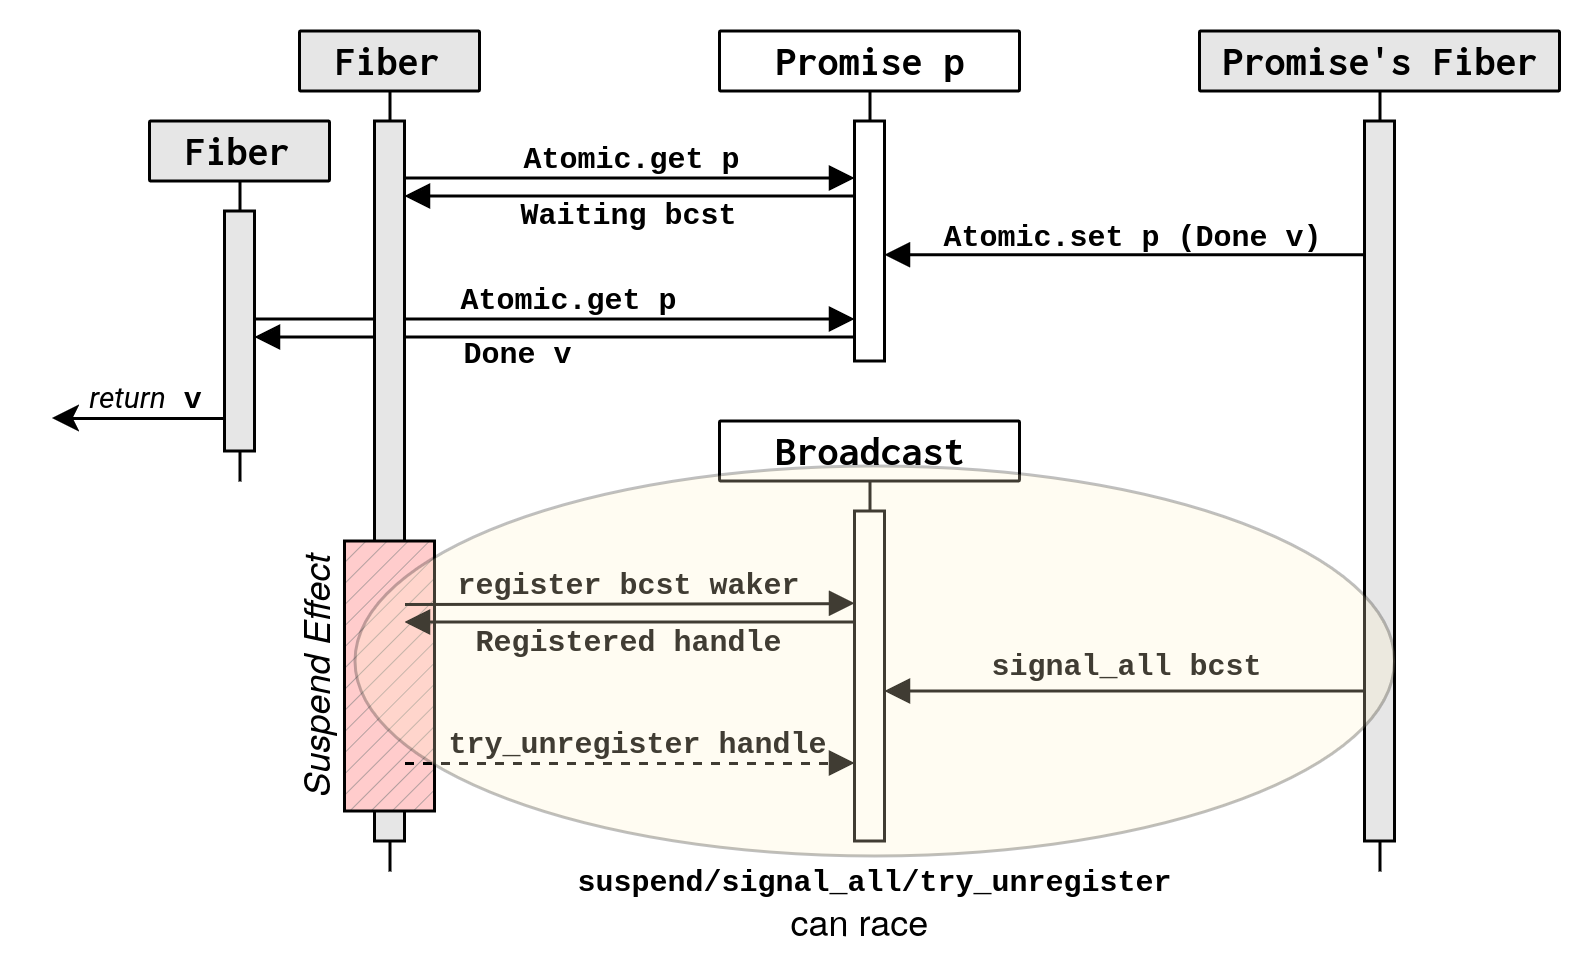
\includegraphics[width=0.75\textwidth]{CQS_Outer_Atomic.png}
  \caption{Usage of CQS with an Outer Atomic Variable}
\end{figure}

It is important to note that since CQS is lock-free and fibers can run on different threads there can be a race between concurrent \textit{suspend}, \textit{cancel} and \textit{signal-all operations}.
Possible interleavings and the necessity of the \textit{cancel operation} are explained in section~\ref{sec:sched-impl-await}.
This example illustrates that a CQS instance always acts as a thread-safe store for cancellable callbacks.
More precisely, it is a FIFO queue but a \textit{signal-all operation} dequeues all elements at once.

% <!-- What are the types of the operations. -->

That CQS is "just" a store for cancellable callbacks is also reflected in the rather barebones types of the operations as implemented in OCaml.
A CQS instance can be \ocamlin{create}d and shared between different threads.
New callbacks are inserted using the \ocamlin{suspend} function, yielding an optional \ocamlin{request} value.
If \ocamlin{suspend} returns \ocamlin{None} the callback has already been invoked due to a concurrent \ocamlin{signal_all}.
A \ocamlin{request} value can then be used to cancel the insertion, signifying that a fiber can only cancel its own callback.
The \ocamlin{signal_all} function (logically) consumes the CQS, which will become more clear when we present the specifications in section~\ref{sec:cqs-spec}.

\begin{figure}[ht]
  \begin{minted}{ocaml}
type t
type request

val create : unit -> t
val suspend : t -> (unit -> unit) -> request option
val cancel : request -> bool
val signal_all : t -> unit
\end{minted}
  \caption{Interface of the CQS Module}
\end{figure}

\subsection{Implementation and Logical Interface of CQS}
\label{sec:cqs-impl}

% <!-- Some general information how CQS is implemented and the logical state describing the entire queue. -->

CQS is implemented as a queue of \textit{cells} with two pointers pointing to the beginning and end of the active cell range, the \textit{suspend pointer} and the \textit{resume pointer}.
Cells not reachable from either pointer are garbage collected but their logical state is still tracked.
There is a stack of operations for manipulating these pointers to implement the higher-level functionality but they are not part of the public API so we do not focus on them.
Each cell is a container for one handle and the logical state of the queue tracks the logical state of all existing cells shown in figure~\ref{fig:cqs-cell-states}.

The number of active cells \ocamlin{n} (i.e. the length of the queue) is tracked by the logical resource \ocamlin{cqs_state n}.
In normal usage of CQS, the atomic variable of the outer synchronization construct would encode the length of the queue in its value and keep this resource in an associated invariant.
Logically changing the length of the queue is done using \textit{enqueue} and \textit{dequeue registration} operations when opening this invariant.

As we saw before, however, for promises the exact length of the queue is irrelevant because the \textit{signal-all operation} will always set the length to 0.
So in the adapted proof we keep the \ocamlin{cqs_state n} resource in the invariant of CQS itself.
As a consequence we also move the \textit{enqueue} and \textit{dequeue registration} out of the public API because they are now done internally.

\subsection{Verification of the \ocamlin{Broadcast} Module}
\label{sec:cqs-spec}

In the following we describe the specifications we proved for the three operations \ocamlin{suspend}, \ocamlin{cancel} and \ocamlin{signal_all} of Eio's \ocamlin{Broadcast} module, in which points they differ from the specifications of the original CQS operations, and what changes we did to the internal logical state of CQS to carry out the proofs.

% <!-- Futures vs. Callbacks -->

The first major change was replacing the future-based interface of the suspend operation with a callback-based interface.
In the original CQS, performing a suspend operation returns a new future, which is also inserted as the handle into the queue.
The execution context can then use the future to stop execution because it is assumed there is a runtime that allows suspending execution until the completion of a future.
But Eio cannot use this interface because it uses the customized CQS to \textit{build} the runtime that allows fibers to suspend until the completion of a promise.
As explained above, Eio implements CQS with a callback-based interface where the fiber performing the suspend operation passes in a callback as the handle and afterwards implicitly stops execution.
Performing a resume operation analogously invokes the callback, instead of completing the future.

This changes the logical state of CQS only slightly.
The original CQS tracked the state of the future for each cell and managed \textit{futureCancellation} and \textit{futureCompletion} tokens.
In the customized CQS we analogously track the state of the callback for each cell and manage \textit{callbackInvokation} and \textit{callbackCancellation} tokens.

For all three operations, the Eio implementation differs from the implementation already verified in the original CQS (i.e. some reordered instructions or a slightly different control flow) and they have different specifications as discussed below.
However, the specifications of the underlying operations for manipulating the cell pointers are modular enough to allow us to prove the new specifications for \ocamlin{suspend} and \ocamlin{cancel}.
Note that the presented specifications are cleaned up for readability.

% Aside: Implementation of signal_all
% Eio implements signal_all by atomically increasing the \textit{resume pointer} by some number n, instead of just 1 like in the original resume.
% Because of technical differences between the infinte array implementation in the CQS mechanization & the infinite array implementation of Eio did not yet verify Eio's custom signal_all function.
% Instead, I actually defined signal_all simply as a loop over a resume operation.
% Since signal_all is only called once I posit that this verification is still valid but I still want to verify Eio's signal_all and remove this aside.

The logical state of an individual cell is changed by the functions according to the following diagram.

\begin{figure}[ht]
  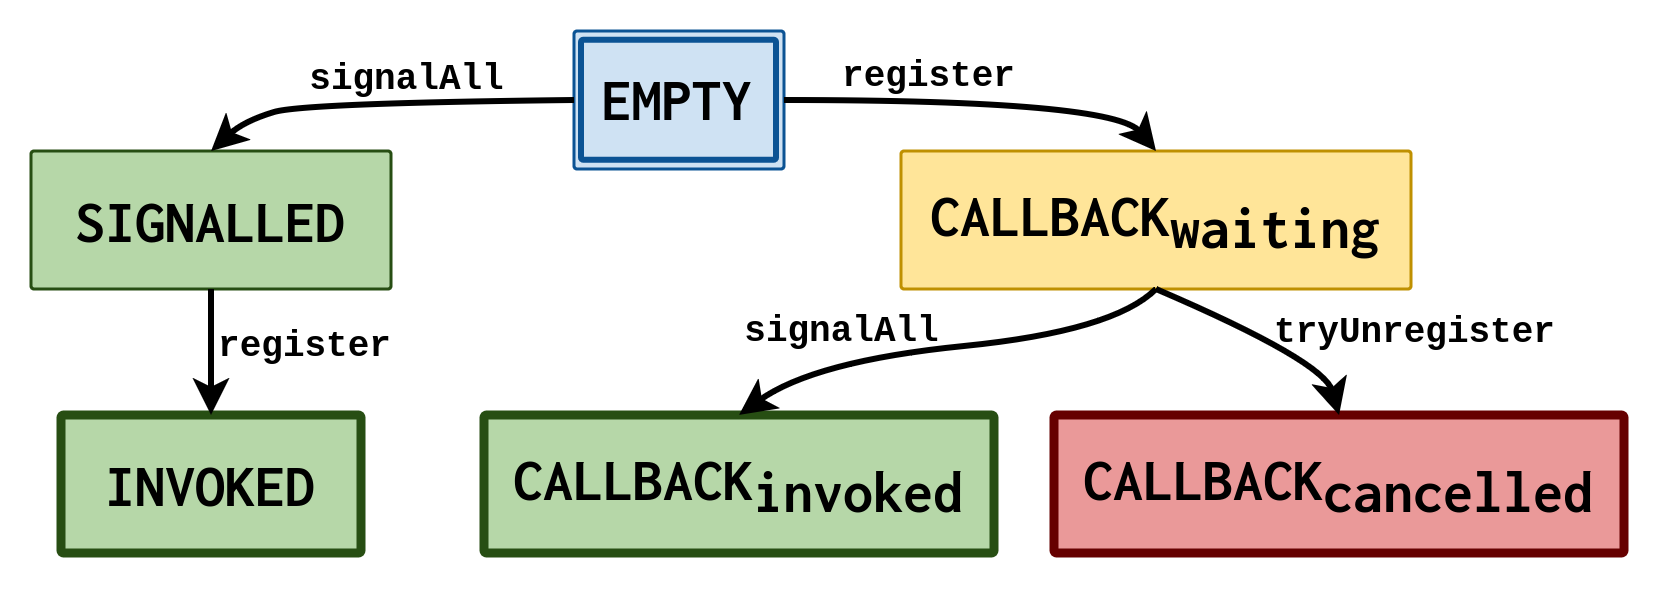
\includegraphics[width=0.75\textwidth]{Cell_States.png}
  \caption{State Transition Diagram for a Single Cell.}
  \label{fig:cqs-cell-states}
\end{figure}

\subsubsection{\ocamlin{create}}
\label{sec:cqs-spec-create}

Creating a CQS instance requires \ocamlin{inv_heap_inv} which is an Iris propositions that we are in a garbage-collected setting.
It creates an \ocamlin{is_cqs γ q} which is a persistent resource that shows the value \ocamlin{q} is a CQS queue, along with a collection of ghost names we summarize with \ocamlin{γ}.
The resource \ocamlin{cqs_state n} mentioned above is now kept inside \ocamlin{is_cqs γ q}.
It also returns the unique resource \gssignal{}, which is held by the enclosing promise and allows calling the \ocamlin{signal_all} function once.

\begin{minted}{coq}
Theorem create_spec:
{{{ inv_heap_inv }}}
newThreadQueue #()
{{{ γ q, RET q; is_cqs γ q ∗ signal_all_permit γ }}}.
\end{minted}

\subsubsection{\ocamlin{suspend}}
\label{sec:cqs-spec-suspend}

For a \textit{suspend operation} the \textit{suspend permit} from the original CQS is not needed anymore since we do the \textit{enqueue registration} internally.
The \ocamlin{is_waker} resource is defined as \ocamlin{V' -∗ EWP k () {{ ⊤ }}} and represents the permission to invoke the callback \ocamlin{k}.
We instantiate \ocamlin{V'} with \ocamlin{promise_state_done γp} so that the callback transports the knowledge that the promise has been fulfilled.
\ocamlin{is_waker} is not persistent because the callback must be invoked only once and it might be accessed from a different thread.

The \ocamlin{suspend} function will advance the \textit{suspend pointer} to allocate a new cell in the \textbf{EMPTY} logical state.
If there is a concurrent call to \ocamlin{signal_all} which changed the cell to the \textbf{RESUMED} logical state before this function can \ocamlin{CAS} the callback into the cell, the callback is invoked immediately and \ocamlin{NONEV} is returned.
In this case, the state of the cell will be set to \textbf{TAKEN}.
Otherwise the callback is saved in the cell, which is advanced to the \textbf{CALLBACK(waiting)} logical state and a \ocamlin{is_suspend_result} resource is returned as the cancellation permit.

\begin{minted}{coq}
Theorem suspend_spec γ q k:
{{{ is_cqs γ q ∗
                is_waker V' k }}}
suspend q k
    {{{ v, RET v; ⌜v = NONEV⌝ ∨
                        ∃ γk r, ⌜v = SOMEV r⌝ ∗
                        is_suspend_result γ γk r k }}}.
\end{minted}

\subsubsection{\ocamlin{cancel}}
\label{sec:cqs-spec-cance}

The specification of the \textit{cancel operation} is a lot simplified compared to the original due to removed features.
The \ocamlin{is_suspend_result} resource is used as a permission token and the \ocamlin{r} value is used to find the callback that should be cancelled.

If the callback had already been invoked by a concurrent call to \ocamlin{signal_all} (i.e. the logical state is \textit{CALLBACK(resumed)}) the function returns \ocamlin{false} and no resources are returned to the caller.
Otherwise, the permission to invoke the callback is returned and the cell is advanced to the \textit{CALLBACK(cancelled)} logical state.

\begin{minted}{coq}
Theorem try_cancel_spec γ q γk r k:
{{{ is_cqs γ q ∗
                is_suspend_result γ γk r k }}}
cancel r
    {{{ (b: bool), RET #b; if b then is_waker V' k
                        else True }}}.
\end{minted}

\subsubsection{\ocamlin{signal_all}}
\label{sec:cqs-spec-signal-all}

The specification of the \textit{signal-all operation} is also a lot simplified compared to the specification of the original \textit{resume operation} because we removed multiple unused features.
The \gssignal{} is a unique resource used to ensure the function can only be called once.
The \ocamlin{V'} resource must be duplicable because it will be used to invoke multiple callbacks, which have \ocamlin{V'} as their precondition.
It does not return any resources because its only effect is making an unknown number of fibers resume execution, which is not something we can easily formalize in Iris.

\begin{minted}{coq}
Theorem signal_all_spec γ q:
{{{ is_thread_queue γ q ∗
                □ V' ∗
                signal_all_permit γ }}}
signal_all q
    {{{ RET #(); True }}}.
\end{minted}

\subsection{Features Removed from Original CQS}
\label{sec:cqs-spec-removed-features}

The original CQS supports multiple additional features like a synchronous mode for suspend and resume, and also a smart cancellation mode.
These features enlarge the state space of CQS and complicate the verification but are not used in Eio so when we ported the verification of CQS to our Eio case study we removed support for these features.
This reduced the state space of a cell shown below (taken from the original paper) to something more manageable for us when adapting the proofs.

\begin{figure}[ht]
  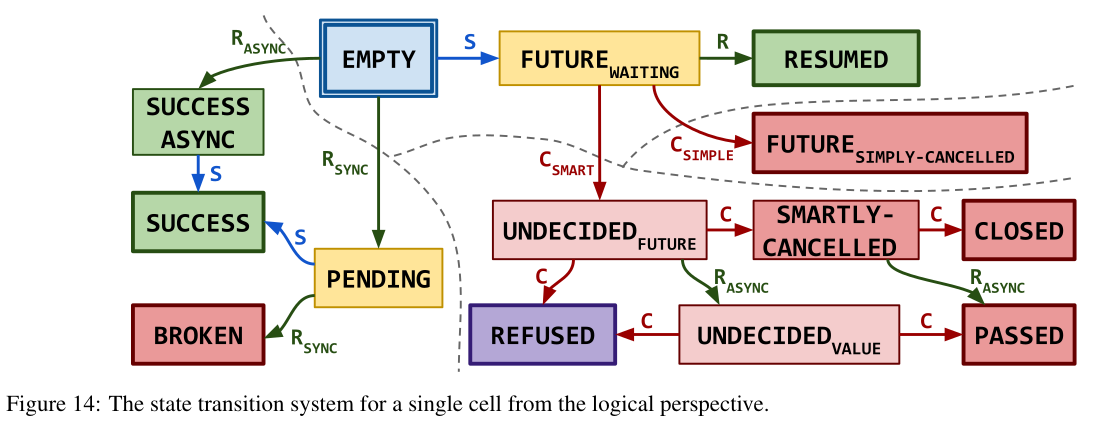
\includegraphics[width=0.75\textwidth]{Cell_States_Original.png}
  \caption{Cell States in the Original CQS}
\end{figure}

Due to this, the part of the verification of the original CQS that we had to customize for Eio shrunk by approximately 1300 lines of Coq code from the original 3600 lines of Coq code, while there is an additional ~4000 lines of Coq code that we did not need to adapt.
